\documentclass[tikz,border=8pt]{standalone}
% Shared look for every TikZ diagram. Load with \input{../../tools/tikz-style.tex}
\usepackage[T1]{fontenc}
\usepackage{lmodern}
\renewcommand{\sfdefault}{lmr}  % diagrams use the same serif as the text
\usetikzlibrary{arrows.meta, positioning, shapes.geometric, calc, fit, backgrounds}
\definecolor{cblue}{HTML}{4C78A8}
\definecolor{corange}{HTML}{F58518}
\definecolor{cgreen}{HTML}{54A24B}
\definecolor{cred}{HTML}{E45756}
\definecolor{cpurple}{HTML}{B279A2}
\definecolor{cgrey}{HTML}{6B6B6B}
\tikzset{
  every picture/.style={font=\sffamily, line width=1.2pt},
  box/.style={draw=#1, fill=#1!12, rounded corners=4pt, align=center, inner sep=7pt, minimum height=1.1cm},
  box/.default=cgrey,
  arrow/.style={-{Stealth[length=3mm]}, draw=cgrey, line width=1.4pt},
  title/.style={font=\sffamily\bfseries\Large},
  note/.style={font=\sffamily\small, text=cgrey, align=center},
}
\AtBeginDocument{\hyphenpenalty=10000 \exhyphenpenalty=10000}

\begin{document}
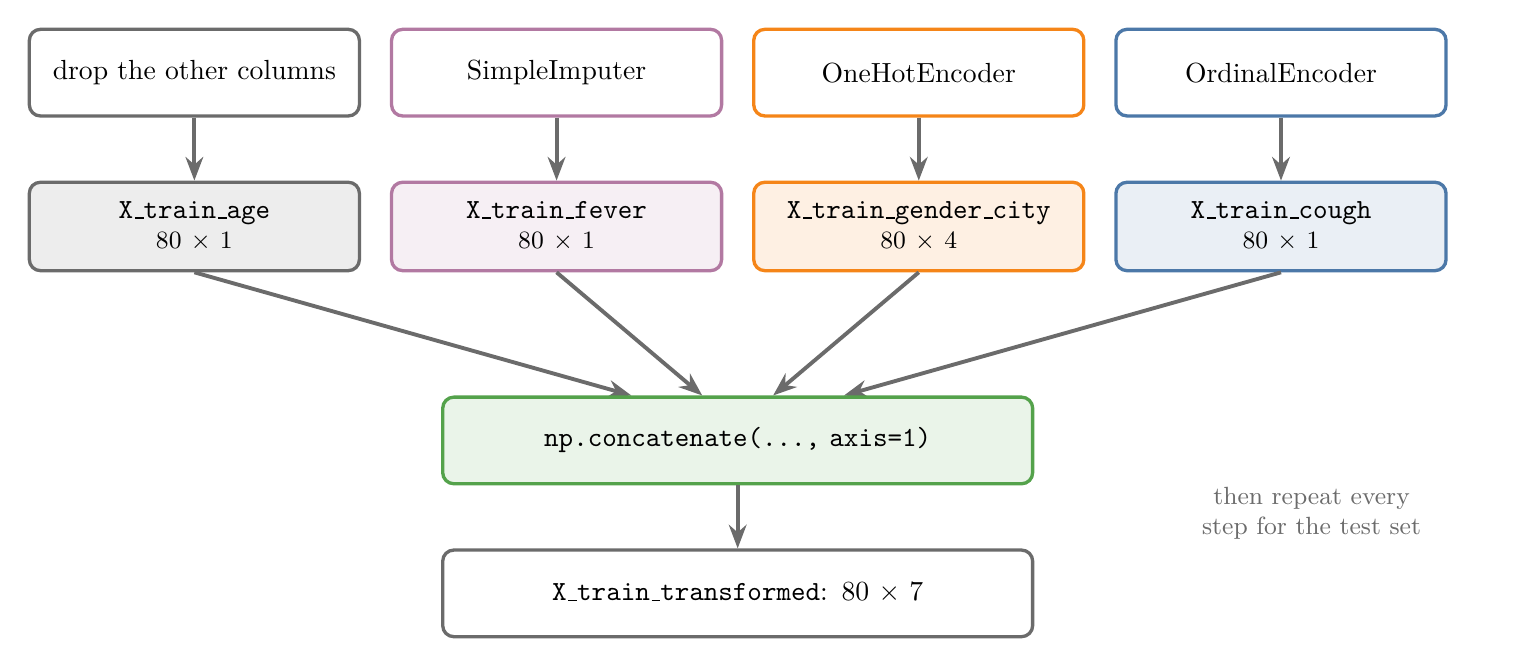
\begin{tikzpicture}
  % step 1: four separate jobs, each giving its own array
  \foreach \i/\c/\job/\arr/\sh/\w in {
      0/cgrey/drop the other columns/X\_train\_age/80 $\times$ 1/1,
      1/cpurple/SimpleImputer/X\_train\_fever/80 $\times$ 1/1,
      2/corange/OneHotEncoder/X\_train\_gender\_city/80 $\times$ 4/4,
      3/cblue/OrdinalEncoder/X\_train\_cough/80 $\times$ 1/1} {
    \node[box=\c, fill=white, text width=3.7cm] (j\i) at (4.6*\i,0) {\job};
    \node[box=\c, text width=3.7cm, below=0.8cm of j\i] (a\i) {\texttt{\arr}\\[-1pt]\small \sh};
    \draw[arrow] (j\i) -- (a\i);
    \draw[arrow] (a\i.south) -- ({6.9+0.9*(\i-1.5)},-4.1);
  }
  \node[box=cgreen, text width=7cm, anchor=north] (cat) at (6.9,-4.1) {\texttt{np.concatenate(..., axis=1)}};
  \node[box=cgrey, fill=white, text width=7cm, below=0.8cm of cat] (out) {\texttt{\textbf{X\_train\_transformed}}: 80 $\times$ 7};
  \draw[arrow] (cat) -- (out);
  \node[note, text width=4.5cm, anchor=west] at (11.8,-5.6) {then repeat every\\step for the test set};
\end{tikzpicture}
\end{document}
